% !TeX root = ../main.tex
\section{子空间, 积空间, 商空间}
\subsection{子空间}
    \begin{Definition}[集族在一个子集上的限制]
        设 $ (X, \ST) $ 是一个拓扑空间, $ Y\subset X $, $ \CA\subset X $ 是 $ X $ 中的一个集族, 称
        \begin{align*}
            \CA|_{Y}=\set{A\cap Y:A\in\CA}=\CA\cap Y
        \end{align*}
        为\emph{集族 $ \CA $ 在 $ Y $ 上的限制}.
    \end{Definition}

    \begin{Definition}[子空间拓扑]
        设 $ (X, \ST) $ 是拓扑空间, $ Y\subset X $, 则 $ \ST|_{Y} $ 是 $ Y $ 的一个拓扑, 称为 $ Y $ 上的\emph{子空间拓扑}.
    \end{Definition}
    
    \begin{Remark}
        度量空间 $ X $ 的子集上, 按 $ X $ 的度量诱导的拓扑与 $ Y $ 的子空间拓扑一致.
    \end{Remark}

    \begin{Proposition}[子空间中集合的拓扑运算]
        设 $ (X, \ST) $ 是一个拓扑空间, $ Y\subset X, A\subset Y $ 则
        \begin{lpbn}(2)
            \task $ \ST_{Y}=\ST|_{Y} $,
            \task $ \SF_{Y}=\SF|_{Y} $,
            \task $ \CN_{Y}(y)=\CN(y)|_{Y} $,
            \task $ d_{Y}(A)=d(A)\cap Y $,
            \task! $ \mathrm{cl}_{Y}(A)=\mathrm{cl}(A)\cap Y $,
            \task! 若 $ \CB $ 是 $ Y $ 的基, 则 $ \CB|_{Y} $ 是 $ Y $ 的基,
            \task! 对 $ y\in Y $, 若 $ \CN(y) $ 是 $ X $ 中 $ y $ 的邻域基, 则 $ \CB(y)|_{Y} $ 是 $ Y $ 中 $ y $ 的邻域基. 
        \end{lpbn}
    \end{Proposition}
    \begin{Proof}
        (1) -- (2) 显然.
        
        (3) 即证互相包含. 
        \begin{align*}
            \forall U\in\CN_{Y}(y)\,\exists V\in\ST_{Y}\,(y\in V\subset U) & \Longrightarrow \exists V_{1}\in\ST\,(V=V_{1}\cap Y)\\
            & \Longrightarrow y\in V_{1}\subset(V_{1}\cup U=:U_{1})\\
            & \Longrightarrow U_{1}\in\CN(y),
        \end{align*}
        又因为
        \begin{align*}
            U_{1}\cap Y=(V_{1}\cup U)\cap Y=V\cup U=U,
        \end{align*}
        即 $ U\in\CN(y)|_{Y} $, 即 $ \CN_{Y}(y)\subset \CN(y)|_{Y} $.

        再证反向不等式.
        \begin{align*}
            \forall U\in\CN(y)|_{Y}\,\exists V\in\CN(y)\,(U=V\cap Y)\Longrightarrow W\in\ST\,(y\in W\subset V),
        \end{align*}
        取 $ W_{1}=W\cap Y $, 则 $ W_{1}\in\ST|_{Y} $. 且
        \begin{align*}
            U=V\cap Y\supset W\cap Y=W_{1}\ni y,
        \end{align*}
        即 $ U\in\CN_{Y}(y) $, 即 $ \CN(y)|_{Y}\subset \CN_{Y}(y) $.

        从而 $ \CN_{Y}(y)=\CN(y)|_{Y} $.
        \begin{figure*}[!htb]
            \centering
            \subfloat[$ \CN_Y(y)\subset\CN(y)|_Y $中的几何关系]{\includegraphics[width=0.35\linewidth]{figures/TopoFig5.png}} \qquad
            \subfloat[$ \CN(y)|_Y\subset\CN_Y(y) $中的几何关系]{\includegraphics[width=0.35\linewidth]{figures/TopoFig6.png}}
        \end{figure*}

        (4) -- (6) 由定义可证.

        (7) 由 (3) 与 (6) 可证.\qed
    \end{Proof}
    
    \begin{Example}
        子空间中的开集未必是原空间上的开集. 例如取 $ \R^{2} $ 上通常的拓扑. 取
        \begin{align*}
            \R^{1}=\set{(x, y)\in\R^{2}: y=0}
        \end{align*}
        上的子空间拓扑. 则 $ (a, b)\times\set{0} $ 在 $ \R^{1} $ 中开. 但不是 $ \R^{2} $ 上的开集. 同样地, 闭集, 闭包, 内部也有类似的反例.
    \end{Example}

\subsection{积空间}
    接下来考虑的对象发生了变化
    \begin{align*}
        \R^{1} & \xlongrightarrow{} \R^{n}:=\R^{1}\times\R^{1}\times\dots\times\R^{1}\\
        (X, \ST) & \xlongrightarrow{} \Prod{i=1}{n}(X_{i}, \ST_{i}):=(X_{1}, \ST_{1})\times(X_{2}, \ST_{2})\times\dotsb\times(X_{n}, \ST_{n}),
    \end{align*}
    Cartesian 积只是集合, 其上不带有任何的结构. 

    \begin{Definition}[乘积拓扑]
        设 $ (X_{i}, \ST_{i}) $ 是拓扑空间. 称 $ p_{j}:\Prod{i\in I}{}X_{i}\to X_{j} $ 是第 $ j $ 个射影. 令
        \begin{align*}
            \CS=\set{p_{j}^{-1}(U_{i}): U_{i}\in\ST_{i}, j\in I},
        \end{align*}
        称 $ \Prod{i\in I}{}X_{i} $ 上以 $ \CS $ 为子基的拓扑 $ \ST $ 为\emph{积拓扑}. $ \left( \Prod{i\in I}{}X_{i}, \ST \right) $ 称为 $ \set{(X_{i}, \ST_{i})}_{i\in I} $ 的\emph{积空间}, 简记作 $ \Prod{i\in I}{} X_{i} $.

        特别地, 若 $ \abs{I}<\infty $, 定义等价于以 $ \CB=\set{\Prod{i\in I}{}U_{i}: U_{i}\in \ST_{i}} $ 为基的拓扑.
    \end{Definition}

    \begin{Example}
        下面给出一些乘积拓扑的例子:
        \begin{enumerate}
            \item 2 -- 环面 $ \T^{2}\cong \T^{1}\times\T^{1} $. 考虑换上经纬度为 $ (x_{1}, x_{2}) $ 的点, 作同胚
            \begin{align*}
                \varphi: & \T^{2} \to \T^{1}\times\T^{1}, \\
                & ((a+\cos x_{2})\cos x_{1}, (a+\cos x_{2})\sin x_{1}, \sin x_{2}) \mapsto (\exp(2\pi\imag x_{1}), \exp(2\pi\imag x_{2}))
            \end{align*}
            \item 刺破的平面 $ \C\sm\set{0}\cong \R^{1}\times\S^{1} $. 考虑非零复数的极坐标表示 $ z=r\exp(\imag\theta) $, 作同胚:
            \begin{align*}
                \varphi: \C\sm \set{0}\to \R^{1}\times \S^{1}, \quad z=r\exp(\imag\theta)\mapsto(\log r, \exp(\imag\theta)).
            \end{align*}
        \end{enumerate}
    \end{Example}

    \begin{Theorem}[射影性质与积拓扑的``最小性'']
        射影 $ p_{j}:\Prod{i\in I}{}X_{i}\to X_{j} $ 是连续的, 满的开映射, 且积拓扑是使所有 $ p_{j} $ 连续的最粗(最弱)的拓扑.
    \end{Theorem}
    \begin{Proof}
        显然 $ p_{j} $ 是满射. 又因为 $ \forall U_{j}\in\ST_{j}\,(p_{j}^{-1}(U_{j})\in\CS\subset\ST) $, 故 $ p_{j} $ 连续. 往证 $ p_{j} $ 是开映射. 为此, 只需 $ \forall B\in\CB\,(p_{j}(B)\in\ST_{j}) $ 即可. 设
        \begin{align*}
            B\bigcap_{k=1}^{n}P_{i_{k}}^{-1}(U_{i_{k}}),
        \end{align*}
        其中 $ U_{i_{k}}\in\ST_{i_{k}} $, 则
        \begin{align*}
            p_{j}(B)=\begin{cases}
                U_{j} & , j\in\set{\seq[k]{i}}\\
                X_{j} & , j\notin\set{\seq[k]{i}}
            \end{cases}\in \ST_{j}
        \end{align*}
        故 $ p_{j} $ 是开映射.

        再设 $ \tilde{\ST} $ 也使各 $ p_{j} $ 连续, 则 $ \forall U_{j}\in\ST_{j}\,(p_{j}^{-1}(U_{j})\in\tilde{\ST}) $. 也即 $ \CS\subset\ST $. 从而 $ \CS $ 生成的积拓扑 $ \ST\subset\tilde{\ST} $.\qed
    \end{Proof}
    
    \begin{Theorem}[连续映射的投影刻画]
        设 $ X_{i}, Y $ 是拓扑空间, 则映射 $ f: Y\to \Prod{i\in I}{}X_{i} $ 连续的充分必要条件是各 $ f_{j}=p_{j}\circ f: Y\to X_{j} $ 连续.
        \begin{center}
            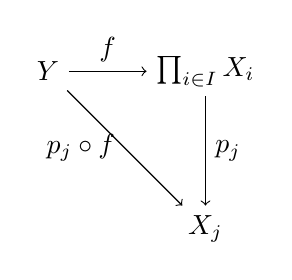
\begin{tikzpicture}
                \node (Y) at (0,0) {$ Y $};
                \node (PX) at (2,0) {$ \prod_{i\in I}X_i $};
                \node (Xj) at (2,-2) {$ X_j $};
                \draw[->] (Y) -- node[above]{$ f $} (PX);
                \draw[->] (PX) -- node[right]{$ p_j $} (Xj);
                \draw[->] (Y) -- node[left]{$ p_j\circ f $} (Xj);
            \end{tikzpicture}
        \end{center}
    \end{Theorem}
    \begin{Proof}
        \textsl{必要性}. 由复合的连续性可得.

        \textsl{充分性}. 若所有 $ p_{j}\circ f $ 连续, 则
        \begin{align*}
            \forall U_{j}\in\ST_{j}\,(p_{j}^{-1}(U_{j})\in\CS\Rightarrow f^{-1}(p_{j}^{-1}(U_{j}))=(p_{j}\circ f)^{-1}(U_{j})\in\ST_{Y}),
        \end{align*}
        即 $ f $ 连续.\qed
    \end{Proof}

\subsection{商空间}

    从等价关系构造商结构, 在拓扑空间即形成商空间. 这是具象的``粘贴''过程的数学描述:

    \begin{Definition}[商空间]
        设 $ (X,\ST) $ 是一个拓扑空间, $ \sim $ 是 $ X $ 上的等价关系, 并记自然射影为 $ \pi : X\to X/\sim $. 商集上的子集族 $ \ST_\sim=\set{U\subset X/\sim : \pi^{-1}(U)\in\ST} $ 是 $ X/\sim $ 上的拓扑, 称作\emph{商拓扑}, 并称 $ (X/\sim,\ST_\sim) $ 称作 $ (X,\ST) $ 关于等价关系 $ \sim $ 的\emph{商空间}.
    \end{Definition}

    \begin{Proposition}
        设 $ X/\sim $ 是 $ X $ 关于 $ \sim $ 的商空间, 则
        \begin{enumerate}
            \item 自然射影 $ \pi : X\to X/\sim $ 是连续满射;
            \item 商拓扑 $ \ST_\sim $ 是使得 $ \sim $ 连续的最细拓扑;
            \item 设 $ Y $ 是拓扑空间, 映射 $ f : X/\sim\to Y $ 连续当且仅当 $ f\circ\pi $ 连续.
        \end{enumerate}
        \begin{center}
            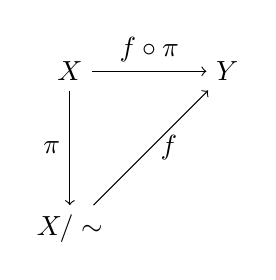
\begin{tikzpicture}
                \node (X) at (0,0) {$ X $};
                \node (Y) at (2,0) {$ Y $};
                \node (X1) at (0,-2) { $ X/\sim $ };
                \draw[->] (X) -- node[above]{$ f\circ \pi $} (Y);
                \draw[->] (X) -- node[left]{$ \pi $} (X1);
                \draw[->] (X1) -- node[right]{$ f $} (Y);
            \end{tikzpicture}
        \end{center}
    \end{Proposition}
    \begin{Proof}
        (1) 满射即商结构的泛性质, 而连续只需注意到任何开集的原像仍然是开的.

        (2) 设 $ \ST' $ 是 $ X/\sim $ 上使得 $ \pi $ 连续的拓扑, 则对任意 $ U\in\ST' $ 有 $ \pi^{-1}(U)\in\ST $. 而由商拓扑的定义可知 $ U\in\ST_\sim $, 于是 $ \ST'\subset\ST_\sim $. 从而 $ \ST_\sim $ 是使得 $ \pi $ 连续的最细的拓扑.

        (3) 必要性显然, 充分性只需考虑 $ f\circ\pi $ 的原像 $ \pi^{-1}(f^{-1}(U)) $ 是 $ X $ 的开集即可.\qed
    \end{Proof}

    商结构的泛性质自然不局限于自然射影 $ \pi $, 对任意 $ f : X\to Y $ 是连续满射, 都可以定义等价关系 $ \sim_f $ 使得 $ x_1\sim x_2 $ 当且仅当 $ f(x_1)=f(x_2) $, 并记 $ f/\sim $ 是在等价类上取值为其代表元上函数值的函数. 上述命题的 (3) 将 $ \pi $ 换成 $ f/\sim $ 后仍然成立.

    \begin{Proposition}
        设 $ f : X\to Y $ 是连续满射, 则 $ f/\sim $ 是连续双射. 且 $ f $ 是开映射或者闭映射时, $ f/\sim $ 是同胚.
    \end{Proposition}

    \begin{Example}
        许多一提到就会令人想到拓扑的形状都可以通过商结构构造出来:
        \begin{enumerate}
            \item 设 $ A $ 是 $ X $ 的闭子集, 若 $ A $ 中所有点同属一个等价类而 $ X\sm A $ 中的每一个点都自成一类, 则得到将 $ A $ 捏成一点构成的空间, 记作 $ X/A $.
            \item 圆环 $ \T^1 $ 可以看作单位区间 $ \mathbb{I}=[0,1] $ 将首尾捏成一点得到的空间 $ \mathbb{I}/\partial\mathbb{I}\simeq\T^1 $, 同胚取 $ p : t\mapsto\exp(2\pi\imag t) $ 导出的 $ p/\sim $ 即可.
            \item 将正方形 $ [0,1]\times[0,1] $ 的两条竖直边反向粘贴, 即 $ (0,x_2)\sim(1,1-x_2) $, 对其他点则自成一等价类. 这样得到的空间即为 \emph{M\"obius 带}.
            \begin{figure}[!htb]
                \centering
                \includegraphics[width=0.4\linewidth]{figures/Mobius_strip.jpg}
            \end{figure}
            \item 将正方形 $ [0,1]\times[0,1] $ 的两条水平边同向粘贴, 再将两条竖直边同向粘贴, 即得到2--环面, 同胚由 $ p: (x_1,x_2)\mapsto(\exp(2\pi\imag x_1),\exp(2\pi\imag x_2)) $ 给出.
            \item 将正方形 $ [0,1]\times[0,1] $ 的两条水平边同向粘贴, 再将两条竖直边同向粘贴, 即得到 \emph{Klein 瓶}.
            \begin{figure}[!htb]
                \centering
                \includegraphics[width=0.25\linewidth]{figures/Klein_bottle.jpg}
            \end{figure}
        \end{enumerate}
    \end{Example}

    \begin{Example}
        还有一个十分重要的例子: \emph{实射影空间} $ \mathbb{RP}^n $: 在 $ X=\R^{n+1}\sm\set{\mathbf{0}} $ 上取等价关系
        \[
            x_1\sim x_2\Longleftrightarrow\exists\lambda\in\R^\times\,(x_1=\lambda x_2),
        \]
        则 $ \mathbb{RP}^n:=X/\sim $. 特别地, $ \mathbb{RP}^2 $ 成为射影平面. 将 $ x\ne 0 $ 所在的等价类对应于 $ \R^{n+1} $ 中过原点 $ \mathbf{0} $ 和 $ x $ 的直线, 就可以将 $ \mathbb{RP}^n $ 看作 $ \R^{n+1} $ 中所有通过原点直线全体.

        设 $ \pi : X\to\mathbb{RP}^n $ 是自然射影, 则 $ \pi $ 在 $ \S^n $ 上的限制 $ p=\pi|_{\S^n} $ 是连续满射, 于是有 $ \mathbb{RP}^n\simeq\S^n/(\sim_p) $. 此时 $ \mathbb{RP}^n $ 可以看作是将 $ \S^n $ 上的 $ x $ 和 $ -x $ 捏成一点得到的空间, $ x $ 和 $ -x $ 称作一对\emph{对径点}.
    \end{Example}